\newpage
\section{Mô hình Bag-of-Words} \label{bow-section}

\paragraph{}{\textbf{Bag-of-Words} (BoW) \cite{qader2019overview} là một dạng biểu diễn đơn giản được sử dụng trong xử lý ngôn ngữ tự nhiên và truy vấn thông tin. 
BoW xem một đoạn văn bản (một câu hoặc một tài liệu) như một "túi" (bag) chứa các từ, hoàn toàn bỏ qua ngữ pháp và thứ tự của các từ, mà chỉ quan tâm đến tần suất xuất hiện của chúng. \\

Nói một cách đơn giản, \textbf{BoW biến một đoạn văn bản thành một danh sách thống kê số lượng của từng từ}. \\

Mô hình BoW chủ yếu được dùng trong các phương pháp phân loại văn bản. Với mô hình này, các đặc trưng dùng để huấn luyện bộ phân loại được tạo ra dựa trên sự xuất hiện hoặc tần suất của mỗi từ trong văn bản.
}

\paragraph{}{Để áp dụng mô hình Bag-of-Words cho một tập hợp nhiều văn bản (gọi là corpus), chúng ta thực hiện các bước sau:}

\begin{enumerate}
    \item \textbf{Tách từ} (Tokenization): Tách các câu thành các từ riêng lẻ (token). Thường thì các dấu câu sẽ bị loại bỏ và các từ được chuyển thành chữ thường.
    \item \textbf{Xây dựng từ điển}: Tạo ra một bộ từ điển chứa tất cả các từ duy nhất xuất hiện trong toàn bộ corpus.
    \item \textbf{Vector hóa} (Vectorization): Với mỗi tài liệu, tạo một vector số. Độ dài của vector này bằng với kích thước của từ điển. Mỗi phần tử trong vector biểu diễn số lần xuất hiện của một từ tương ứng trong từ điển.
\end{enumerate}

\paragraph{}{Kết quả là chúng ta đã chuyển đổi thành công văn bản thành các vector số mà máy tính có thể hiểu và xử lý.}

\begin{figure}[H]
    \centering
    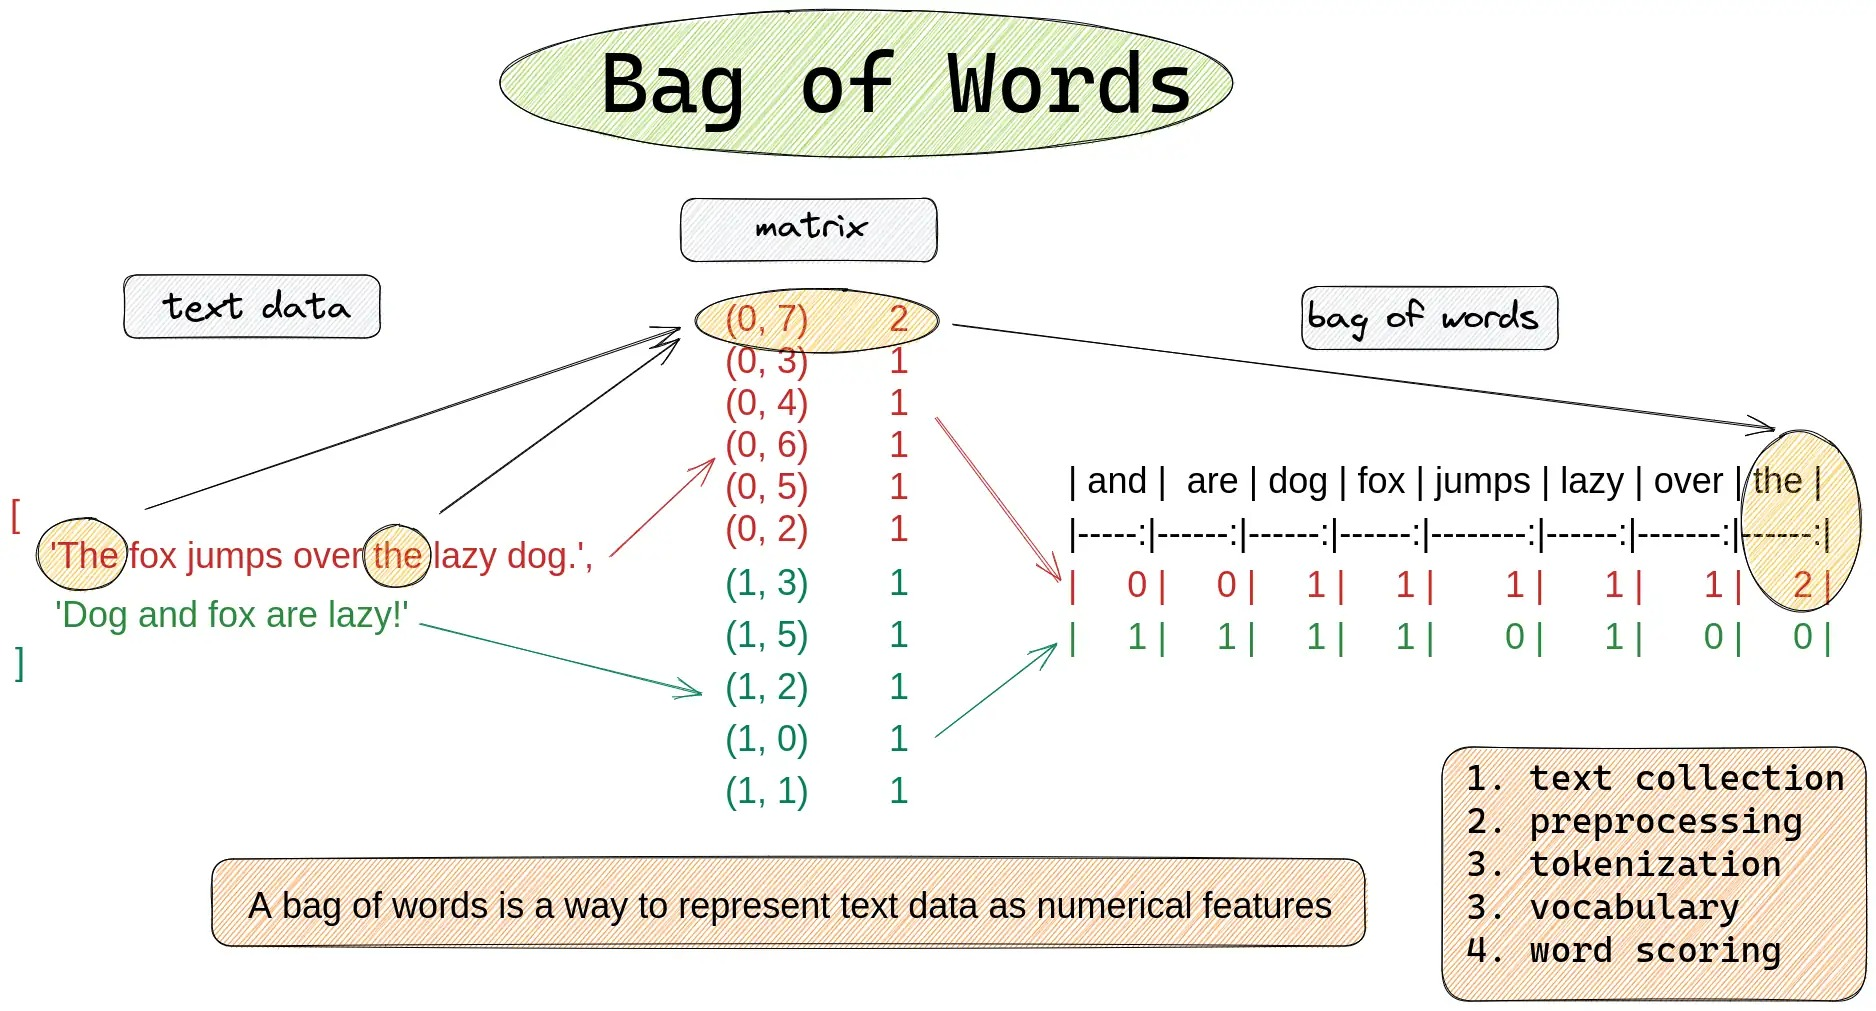
\includegraphics[width=0.84\linewidth]{img/04-bow.jpg}
    \caption{Minh họa mô hình Bag-of-Words}
\end{figure}